\chapter{Diseño e implementación} % Main chapter title

\label{Chapter3} % Change X to a consecutive number; for referencing this chapter elsewhere, use \ref{ChapterX}

\definecolor{mygreen}{rgb}{0,0.6,0}
\definecolor{mygray}{rgb}{0.5,0.5,0.5}
\definecolor{mymauve}{rgb}{0.58,0,0.82}

%%%%%%%%%%%%%%%%%%%%%%%%%%%%%%%%%%%%%%%%%%%%%%%%%%%%%%%%%%%%%%%%%%%%%%%%%%%%%
% parámetros para configurar el formato del código en los entornos lstlisting
%%%%%%%%%%%%%%%%%%%%%%%%%%%%%%%%%%%%%%%%%%%%%%%%%%%%%%%%%%%%%%%%%%%%%%%%%%%%%
\lstset{ %
  backgroundcolor=\color{white},   % choose the background color; you must add \usepackage{color} or \usepackage{xcolor}
  basicstyle=\footnotesize,        % the size of the fonts that are used for the code
  breakatwhitespace=false,         % sets if automatic breaks should only happen at whitespace
  breaklines=true,                 % sets automatic line breaking
  captionpos=b,                    % sets the caption-position to bottom
  commentstyle=\color{mygreen},    % comment style
  deletekeywords={...},            % if you want to delete keywords from the given language
  %escapeinside={\%*}{*)},          % if you want to add LaTeX within your code
  %extendedchars=true,              % lets you use non-ASCII characters; for 8-bits encodings only, does not work with UTF-8
  %frame=single,	                % adds a frame around the code
  keepspaces=true,                 % keeps spaces in text, useful for keeping indentation of code (possibly needs columns=flexible)
  keywordstyle=\color{blue},       % keyword style
  language=[ANSI]C,                % the language of the code
  %otherkeywords={*,...},           % if you want to add more keywords to the set
  numbers=left,                    % where to put the line-numbers; possible values are (none, left, right)
  numbersep=5pt,                   % how far the line-numbers are from the code
  numberstyle=\tiny\color{mygray}, % the style that is used for the line-numbers
  rulecolor=\color{black},         % if not set, the frame-color may be changed on line-breaks within not-black text (e.g. comments (green here))
  showspaces=false,                % show spaces everywhere adding particular underscores; it overrides 'showstringspaces'
  showstringspaces=false,          % underline spaces within strings only
  showtabs=false,                  % show tabs within strings adding particular underscores
  stepnumber=1,                    % the step between two line-numbers. If it's 1, each line will be numbered
  stringstyle=\color{mymauve},     % string literal style
  tabsize=2,	                   % sets default tabsize to 2 spaces
  title=\lstname,                  % show the filename of files included with \lstinputlisting; also try caption instead of title
  morecomment=[s]{/*}{*/}
}

En éste capítulo se describe la estructura de la solución adoptada y el funcionamiento del hardware, software y firmware desarrollado específicamente para el cumplimiento de los requerimientos del sistema.

\section{Solución adoptada}

En base a los requerimientos enumerados en el capítulo 2, se desarrolló un sistema utilizando las tecnologías indicadas en la tabla [\ref{tab:solucionadoptada}].

\begin{table}[h]
	\centering
	\caption[Solución adoptada]{Tecnologías utilizadas en el desarrollo del sistema}
	\begin{tabular}{l m{4.5cm} m{4.5cm}}    
		\toprule
		\textbf{}  					& \textbf{Nodo}     				& \textbf{Gateway}	\\
		\midrule
		Aplicación 					& \ Firmware en C/C++				& \ Firmware en C/C++ y software en Python. \\
		Sistema operativo	 		& \ No corresponde 					& \ Linux\\
		Hardware		 			& \ ESP32(Xtensa LX6) 				& \ Raspberry pi 3(Cortex-A53) y ESP32(Xtensa LX6)\\
		\bottomrule
		\hline
	\end{tabular}
	\label{tab:solucionadoptada}
\end{table}

Se implementó el hardware del nodo en una placa de circuito impreso de diseño específico, descrito en la sección \ref{sec:nodos}. Contiene un microcontrolador de arquitectura MIPS({\textit{Microprocessor without Interlocked Pipeline Stages}}) de 32 bits. Cada nodo posee un circuito integrado de comunicación LoRa con su respectiva antena, sensores y actuadores, ésta permanece a la espera de recepción de comandos, conforme al protocolo propietario desarrollado.

Además se utilizó una raspberry pi como gateway descrito en la seccion \ref{sec:gateway}, a la cual se le conecta un hardware similar al nodo para utilizarlo como transceptor LoRa. La raspberry corre el sistema operativo Linux en la tarjeta microSD. También se desarrolló una aplicación en Python como {\textit{Backend}} de la interfaz web creada en {\textit{Node-red}}.


%----------------------------------------------------------------------------------------
%	SECTION 1
%----------------------------------------------------------------------------------------
\section{Arquitectura de funcionamiento}

En ésta sección se explica la arquitectura utilizada para la comunicación inalámbrica del sistema.
Se toma como referencia la arquitectura distribuida descrita en la sección \ref{sec:arquitecturadedomotica}. Ésta indica que la toma de decisiones por parte del sistema se encuentra en todos los dispositivos, no solo en uno central.
En la figura [\ref{fig:diagramadesecuencia}] se muestra el diagrama de secuencia del sistema. Éste se encuentra montado sobre una red inalámbrica local que utiliza el protocolo LoRa entre gateway y los nodos.

\begin{figure}[ht!]
	\centering
	\includegraphics[width=0.8\textwidth]{./Figures/diagramadesecuencia.png}
	\caption{Diagrama de secuencia del sistema.}
	\label{fig:diagramadesecuencia}
\end{figure}

La arquitectura utilizada posee dos acciones posibles, estas son {\textit{Set}} y {\textit{Get}}. El objetivo de esta arquitectura es la de poder recibir datos con el comando {\textit{Get}} y configurar parámetros con el comando {\textit{Set}}, de ésta manera el sistema se reduce a una arquitectura simple y elemental que no genera grandes complicaciones en la programación de los dispositivos.
En este sistema, cuando existe un nodo o una red de nodos, el gateway se encuentra enviando el comando {\textit{Get}} a cada nodo en intervalos de 20 segundos. Ésto permite que la interfaz web se actualice constantemente. Al no ser un sistema crítico no se necesitan tiempos de respuesta rápidos por lo que 20 segundos es un tiempo prudente.
El nodo tiene permitido enviar datos sin antes haber recibido el comando {\textit{Get}}, solo cuando está en modo automático y tiene activado el sensor de movimiento.


%La idea de esta sección es resaltar los problemas encontrados, los criterios utilizados y la justificación de las decisiones que se hayan tomado.
%
%Se puede agregar código o pseudocódigo dentro de un entorno lstlisting con el siguiente código:
%
%\begin{verbatim}
%\begin{lstlisting}[caption= "un epígrafe descriptivo"]
%	las líneas de código irían aquí...
%\end{lstlisting}
%\end{verbatim}
%
%A modo de ejemplo:
%
%\begin{lstlisting}[label=cod:vControl,caption=Pseudocódigo del lazo principal de control.]  % Start your code-block
%
%#define MAX_SENSOR_NUMBER 3
%#define MAX_ALARM_NUMBER  6
%#define MAX_ACTUATOR_NUMBER 6
%
%uint32_t sensorValue[MAX_SENSOR_NUMBER];		
%FunctionalState alarmControl[MAX_ALARM_NUMBER];	//ENABLE or DISABLE
%state_t alarmState[MAX_ALARM_NUMBER];						//ON or OFF
%state_t actuatorState[MAX_ACTUATOR_NUMBER];			//ON or OFF
%
%void vControl() {
%
%	initGlobalVariables();
%	
%	period = 500 ms;
%		
%	while(1) {
%
%		ticks = xTaskGetTickCount();
%		
%		updateSensors();
%		
%		updateAlarms();
%		
%		controlActuators();
%		
%		vTaskDelayUntil(&ticks, period);
%	}
%}
%\end{lstlisting}

\section{Nodos}
\label{sec:nodos}

El nodo es el dispositivo del sistema del cual se extrae la información de los sensores y se utilizan sus actuadores para generar cambios en dispositivos externos al sistema inalámbrico como ser un aire acondicionado. En esta sección se explicara el hardware y parte del firmware del nodo.

\subsection{Hardware}

El hardware del nodo contiene los siguientes componentes:

\begin{enumerate}
\item Una fuente AC-DC de 220v a 5v. Figura [\ref{fig:esquematico1}].
\item Sensor de temperatura y humedad. Figura [\ref{fig:esquematico2}].
\item Modulo Heltec LoRa v2 con antena adaptada a 915MHz. Figura [\ref{fig:esquematico3}].
\item Circuito de leds infrarrojos. Figura [\ref{fig:esquematico4}].
\item Circuito relay. Figura [\ref{fig:esquematico5}].
\item Circuito de pulsadores. Figura [\ref{fig:esquematico6}].
\item Circuito de leds indiciadores. Figura [\ref{fig:esquematico7}].
\end{enumerate}

En la figura [\ref{fig:esquematico1}] se tiene el circuito de la fuente. Se decidió buscar en el mercado una fuente compacta y pequeña debido al tamaño final que debe tener el producto. Se utilizó la fuente compacta HLK-PM01 de la empresa Hi-Link.

\begin{figure}[h!]
	\centering
	\includegraphics[width=0.6\textwidth]{./Figures/esquematico1.png}
	\caption{Circuito de fuente AC-DC.}
	\label{fig:esquematico1}
\end{figure}

En la figura [\ref{fig:esquematico2}] se muestra el circuito del sensor de temperatura y humedad. El sensor es el conocido DHT11 que tiene un rango de temperatura de 0 a 50 ºC con 5\% de precisión y un rango de humedad de 20 al 80 \% con una precisión del 5\%.

\begin{figure}[h!]
	\centering
	\includegraphics[width=0.6\textwidth]{./Figures/esquematico2.png}
	\caption{Circuito de sensor de temperatura.}
	\label{fig:esquematico2}
\end{figure}

En la figura [\ref{fig:esquematico3}] se ve el circuito de conectores que ofician de zócalo para conectar el modulo externo Heltec LoRa v2. Éste módulo fue elegido debido a que ofrece un microcontrolador esp32 de arquitectura Tensilica Xtensa LX6 de 32bits por lo que se utiliza como controlador principal del nodo, además posee un display oled y el circuito integrado {\textit{SX1276}} de la empresa Semtech, con conector Hirose U.FL para antenas miniatura de RF de hasta 6 GHz.

\begin{figure}[h!]
	\centering
	\includegraphics[width=0.6\textwidth]{./Figures/esquematico3.png}
	\caption{Conectores para el modulo Heltec LoRa v2.}
	\label{fig:esquematico3}
\end{figure}

En la figura [\ref{fig:esquematico4}] se ve un circuito típico para el uso de leds en general. Se utilizaron dos leds debido a que en las pruebas se obtuvo mayor alcance del haz infrarrojo con respecto a los aires acondicionados. El led infrarrojo es el actuador para el encendido y apagado de los aires acondicionados.

\begin{figure}[h!]
	\centering
	\includegraphics[width=0.4\textwidth]{./Figures/esquematico4.png}
	\caption{Circuito de leds infrarrojos.}
	\label{fig:esquematico4}
\end{figure}

En la figura [\ref{fig:esquematico5}] se tiene un circuito típico de relay con su respectivo conector de salida. El relay es el actuador para el encendido y apagado de la luz.

\begin{figure}[h!]
	\centering
	\includegraphics[width=0.6\textwidth]{./Figures/esquematico5.png}
	\caption{Circuito de relay.}
	\label{fig:esquematico5}
\end{figure}

En la figura [\ref{fig:esquematico6}] se muestra el circuito de los pulsadores, éstos son el pulsador de {\textit{Modo}} que se utiliza para sincronizar el nodo con el gateway y además para cambiar el modo de manual a automático, y el pulsador para encendido y apagado de la luz.

\begin{figure}[h!]
	\centering
	\includegraphics[width=0.5\textwidth]{./Figures/esquematico6.png}
	\caption{Circuito de pulsadores.}
	\label{fig:esquematico6}
\end{figure}

En la figura [\ref{fig:esquematico7}] se muestra el circuito de leds indicadores, se utilizan para debugging del sistema.

\begin{figure}[h!]
	\centering
	\includegraphics[width=0.4\textwidth]{./Figures/esquematico7.png}
	\caption{Circuito de leds indicadores.}
	\label{fig:esquematico7}
\end{figure}

La imagen renderizada de la placa de circuito impreso desarrollada en la herramienta libre Kicad, se muestra en la figura [\ref{fig:pcb1}].

\begin{figure}[h!]
	\centering
	\includegraphics[width=0.6\textwidth]{./Figures/pcb1.png}
	\caption{Render de placa de circuito impreso.}
	\label{fig:pcb1}
\end{figure} 

En la figura [\ref{fig:pcb2}] se puede ver la imagen de la pcb realizada. Ésta es una pcb de doble capa, realizada de forma casera con el método de insolación ultravioleta.

\begin{figure}[h!]
	\centering
	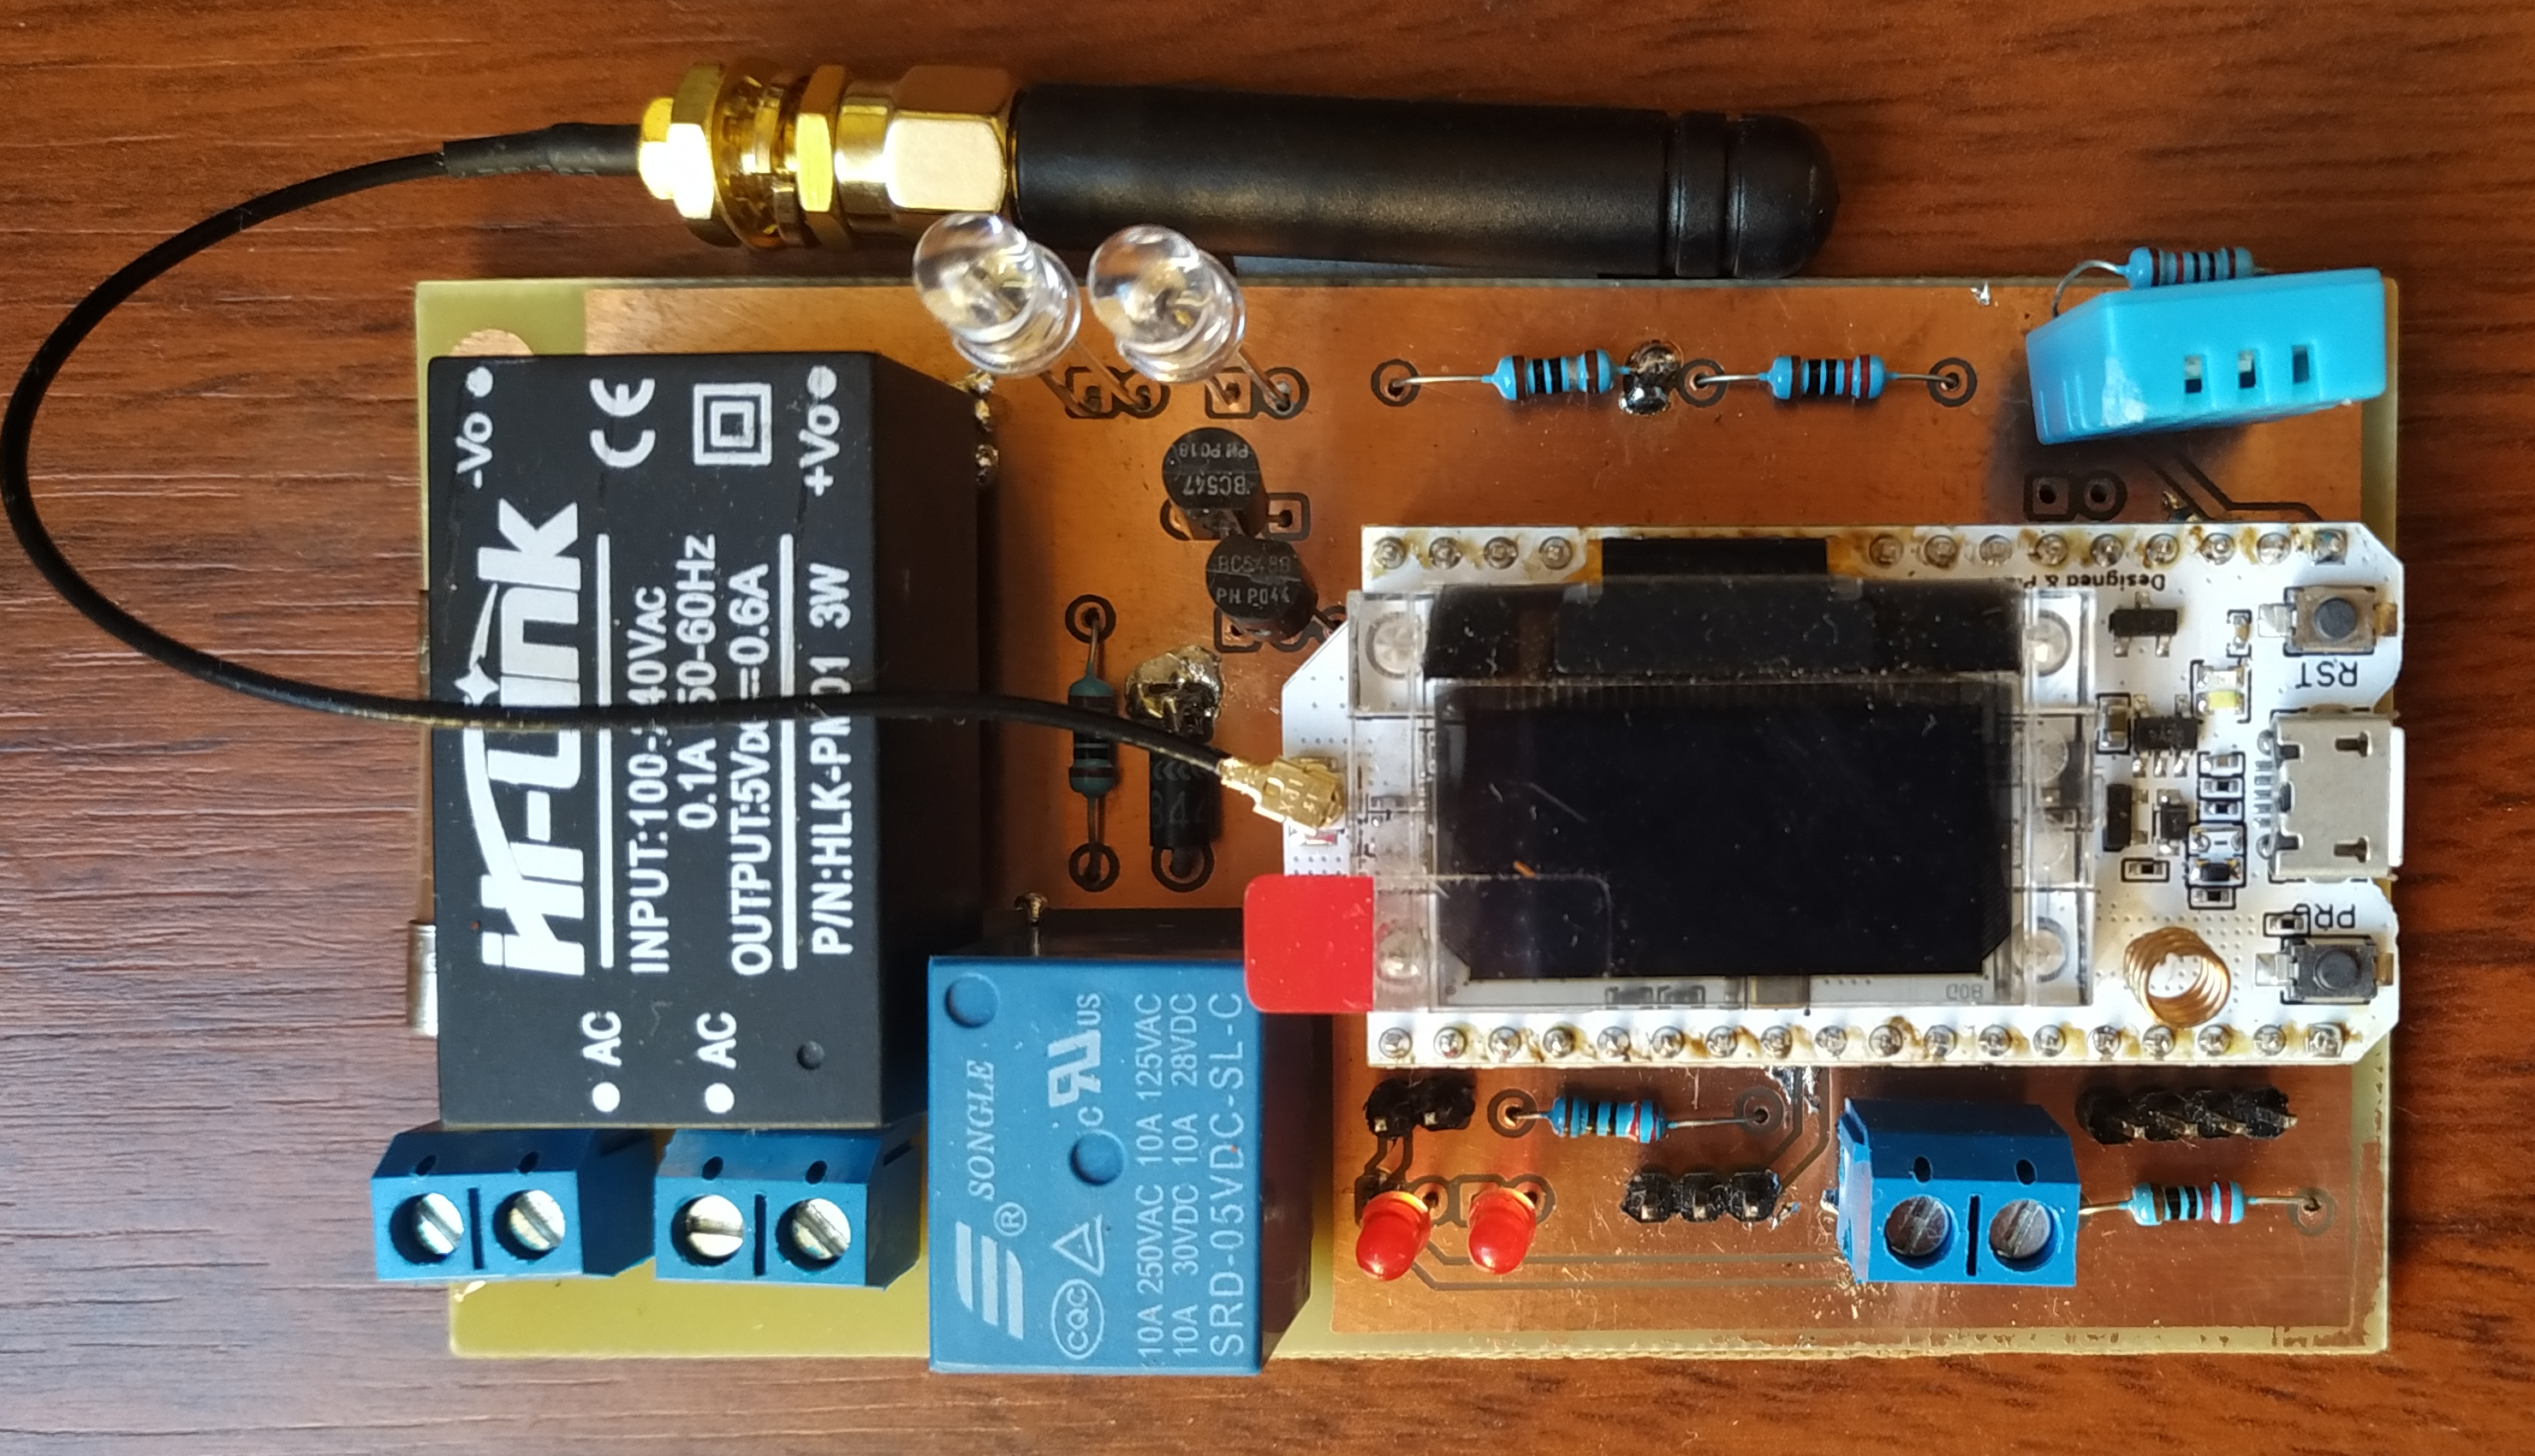
\includegraphics[width=0.6\textwidth]{./Figures/pcb2.png}
	\caption{Placa de circuito impreso.}
	\label{fig:pcb2}
\end{figure} 

\subsection{Firmware}

La arquitectura del firmware se diseño teniendo en cuenta algunos patrones de diseño de arquitectura y conceptos de programación orientada a objetos en C/C++.
Para el desarrollo del firmware se utilizó la API que provee el fabricante del módulo Heltec LoRa, éste provee los drivers de la siguiente lista:

\begin{itemize}
\item Display Oled 128x64.
\item Protocolo LoRa.
\end{itemize}

Además se utilizó una librería creada para el uso de infrarrojos con el microcontrolador ESP32, con el objetivo de agilizar el desarrollo ya que existe una gran variedad de aires acondicionados y protocolos muy variados. Se encontró que la librería provee 92 protocolos, es decir, 92 dispositivos distintos a los cuales se los puede manipular con infrarrojo. Si bien la API de la empresa {\textit{Espressif}}(ESP-IDF), está desarrollada completamente sobre el sistema operativo de tiempo real freeRTOS. Se utilizó como API principal la de Arduino debido a que el sistema no necesita ser de tiempo real, ésta provee soluciones que agilizan el desarrollo de este tipo de dispositivos.

El firmware posee un arquitectura en capas, esto permite la separación de las partes que componen el sistema. En la figura [\ref{fig:capas}] se pueden ver las capas que componen el sistema.

\begin{figure}[h!]
	\centering
	\includegraphics[width=0.6\textwidth]{./Figures/capas.png}
	\caption{Arquitectura en capas del firmware del nodo.}
	\label{fig:capas}
\end{figure}












\section{Gateway}
\label{sec:gateway}

blablaba

\section{Interfaz web}

blabla

\section{Backend del sistema}

blabla

